\documentclass[border=5pt]{standalone}
\usepackage{pgfplots}
\pgfplotsset{compat=1.18}
\begin{document}
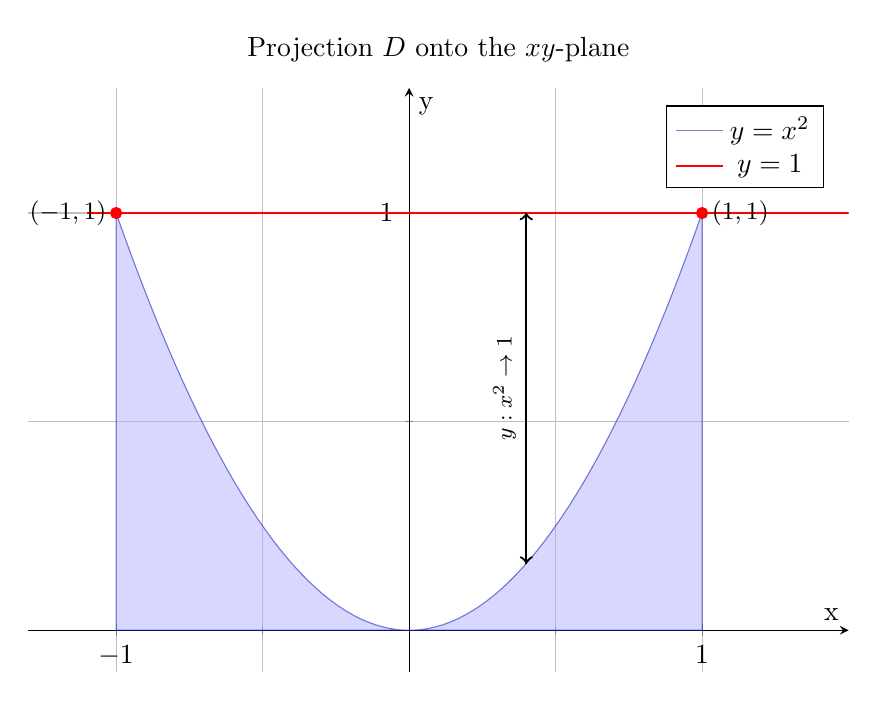
\begin{tikzpicture}
\begin{axis}[
    xlabel={x}, ylabel={y},
    xmin=-1.3, xmax=1.5, ymin=-0.1, ymax=1.3,
    axis lines=middle, xtick={-1,0,1}, ytick={0,1},
    width=12cm, height=9cm,
    grid=both, minor tick num=1,
    title={Projection $D$ onto the $xy$-plane},
    legend style={at={(0.97,0.97)}, anchor=north east}
]
% Shaded region
\addplot[draw=blue!70!black, fill=blue!30, opacity=0.5, domain=-1:1, samples=80]
    {x^2} \closedcycle;
\addplot[draw=red, thick] coordinates {(-1.1,1) (1.5,1)};
\addlegendentry{$y=x^2$}
\addlegendentry{$y=1$}

% Vertical strip indicator
\addplot[black, dashed, thick] coordinates {(0.4,0.16) (0.4,1)};
\draw[<->, thick] (0.4,0.16) -- (0.4,1) node[midway, sloped, above, font=\footnotesize] {$y:x^2\to 1$};

% Intersection points
\addplot[only marks, mark=*, red] coordinates {(1,1) (-1,1)};
\node[anchor=west, font=\small] at (axis cs:1,1) {$(1,1)$};
\node[anchor=east, font=\small] at (axis cs:-1,1) {$(-1,1)$};
\end{axis}
\end{tikzpicture}
\end{document}